\section{Other related methods}

\subsection{Fourier Continuation}

\cite{ganeshram2025fcpinohighprecisionphysicsinformed} use the Fourier Continuation (FC) method to enhance Physics-Informed Neural Operators (PINO) Neural Networks. FC allows to leverage spectral differentiation on non-periodic functions. Spectral differentiation has important advantages against Finite Differences and Automatic Differentiation methods because is can be computed using the Fast Fourier Transform (FFT) algorithm, leading to accurate results even for low-resolution grids and low memory consumption. Fourier Continuation is illustrated in Figure~\ref{fig:FC}.

\begin{figure}[htbp]
  \centering
  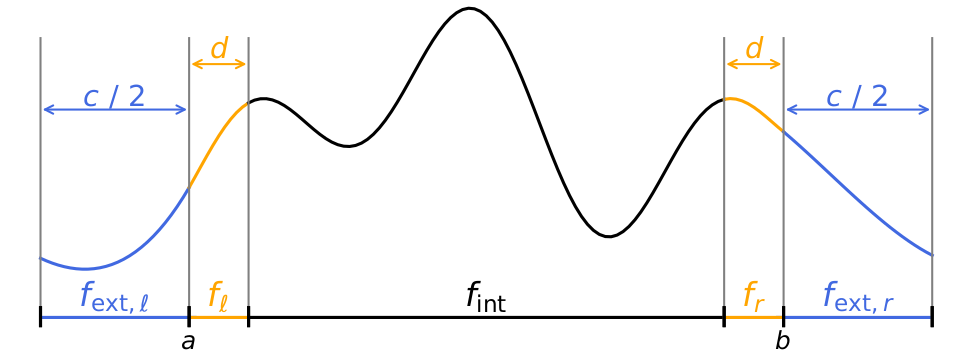
\includegraphics[width=0.4\textwidth]{figures/FC.png}
  \caption{Fourier Continuation applied to a 1D signal}
  \label{fig:FC}
\end{figure}

\noindent A 1D signal $f = [f_l, f_{int}, f_r]$ is extended from domain $[a, b]$ to $[a - \frac{c}{2}, b + \frac{c}{2}]$ :
\begin{align*}
    \tilde{f} = [f_{ext, l}, f, f_{ext, r}]
\end{align*}
\noindent Authors provides 2 methods for computing $f_{ext}^T = (f^T_{ext, l}, f^T_{ext,r})$;
\begin{align*}
     f_{LEGENDRE} & = E \begin{pmatrix}
     f_r \\
     f_l
     \end{pmatrix} \\
     f_{GRAM} = A_lQ^T_lf_l + A_rQ^T_rf_r
\end{align*}
Where the projection matrix $E$, as well as Gram and Continuation matrices $Q_l$, $Q_r$, $A_l$, $A_r$ are described in Appendix~B 1.1 of \cite{ganeshram2025fcpinohighprecisionphysicsinformed}.

\noindent Can FC-PINO be applied to image generation ? There are some 2D and 3D examples in \cite{ganeshram2025fcpinohighprecisionphysicsinformed} (2D viscous Burger Equation, 3D Navier-Strokes Equation). However, they apply FC to every dimension of the input (see their Figure 1). I conjecture that we only need to apply FC to the time dimension of our trajectories. It's unclear on which dimensions should FC be applied for the spectral differentiation of trajectory generation. \\

At the same time, this demonstrates a pit between PINO and image generation models that we can leverage. 

\subsection{REPA : Representation Alignment for Generation}

\cite{yu2025representationalignmentgenerationtraining} build upon the Diffusion-Transformer architecture DiT of \cite{peebles2023scalablediffusionmodelstransformers} (see Figure~\ref{fig:DIT}), where an input is patchified, reshaped to a 1D sequence of patches with a length N, and then fed to the model. Their improvement uses latent diffusion from \cite{DBLP:journals/corr/abs-2112-10752}, which involves learning a latent diffusion $p(\mathbf{z})$, where $\mathbf{z} = E(\mathbf{x})$ is obtained using pre-trained Variational Auto-Encoder (VAE). \\

\begin{figure}[htbp]
  \centering
  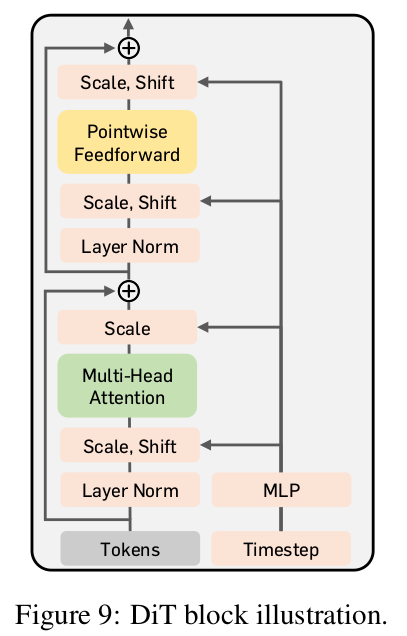
\includegraphics[width=0.4\textwidth]{figures/DiT.png}
  \caption{The DiT block architecture}
  \label{fig:DIT}
\end{figure}

They are aligning representations of the model's hidden state with self-supervised representations. The hidden states $\mathbf{h}_t$ are projected through a projection head $h_{\phi}(\mathbf{h}_t)$, then compared to an encoding from a clean image $\mathbf{z}^{\star} = E(\mathbf{x}^{\star})$. The formalize the following loss:

\begin{align*}
    \mathcal{L}_{REPA}(\theta, \phi) := - \mathbb{E}\left[ \frac{1}{N} \sum_{n=1}^N d(\mathbf{z}^{\star}_n, h_{\phi}(\mathbf{h}_{n, t}))\right]
\end{align*}

\noindent That they integrate into the main loss using a scalar $\lambda$. \\

\noindent In their experiments, they show that their REPA model can significantly enhance the performance of a regular DiT model, while lowering the training time by 17.5. \\

This study highlights another 2 branches of work that we have not yet explored : DiT architecture and latent diffusion. It could be worth reading \cite{peebles2023scalablediffusionmodelstransformers} and \cite{DBLP:journals/corr/abs-2112-10752} to gain a broader understanding of diffusion models. \\

Could we encode the trajectory to predict $\{\mathbf{x}_t\}$ to a smaller dimensionality, especially, compressing the time dimensionality ?

\subsection{Consistency Models Made Easy}

In \cite{geng2024consistencymodelseasy}, the authors generalize diffusion models as a special case of Consistency Models, where the consistency condition:
\begin{align*}
f(\mathbf{x}_t) & = \mathbf{x}_0 \Leftrightarrow \frac{df}{dt} = 0 \\
f(\mathbf{x}_0, 0) & = \mathbf{x}_0
\end{align*}
\noindent is loose. \\

\noindent They introduce the "Curse of consistency" (see Figure~\ref{fig:curse}) by bounding the error:
\begin{align*}
    \lVert f(\mathbf{x}_t) - \mathbf{x}_0 \rVert \leq N e_{max}
\end{align*}
\noindent With $N$ is the number of discretized timesteps, and $e_{max} = \lVert f(\mathbf{x}_{t, i}) - \mathbf{x}_{0, i} \rVert$. They argue that it's hard to lower both $N$ and $e_{max}$ : 
\begin{itemize}
    \item If $N$ is low, then $\Delta t$ is high, and so is $e_{max}$ due to discretization errors.
    \item If $N$ is high, then $\Delta t$ and $e_{max}$ are low.
\end{itemize}

\begin{figure}[htbp]
  \centering
  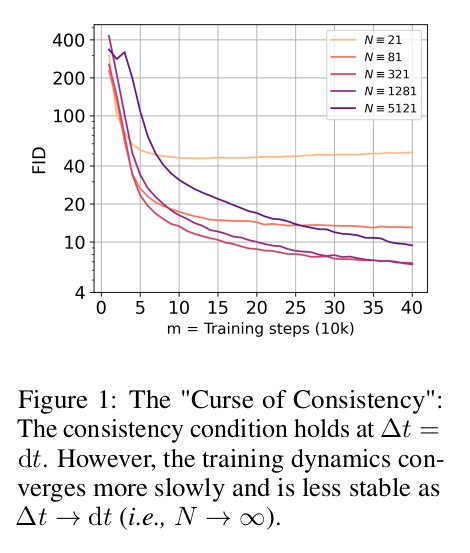
\includegraphics[width=0.4\textwidth]{figures/curse.png}
  \caption{The Curse Of Consistency illustrated.}
  \label{fig:curse}
\end{figure}

\noindent They propose to gradually lower $\Delta t$ during training, setting:
\begin{align*}
    \Delta t &= t - r \\
    \frac{r}{t} &= 1 - \frac{1}{q^{\frac{n}{d}}} \left(1 + \frac{k}{e^{bt}} \right)
\end{align*}
\noindent They remark that when training ($n = 0$), then $\frac{r}{t} = 0$ and this is equivalent to having a regular diffusion training, without consistency. This can be seen as "enforcing the consistency condition as training progresses". \\

\noindent This paper is interesting because it addresses the discretization paradox that we face: more timesteps (larger $N$) lead to potentially smaller errors but are harder to train and less stable; smaller $N$ is easier to train and more stable but also leads to higher errors. \\

\noindent In our case; I guess we need to fix N anyway, because it controls the size of the network's output. Or, we could ignore some steps at the start of training (only computing the loss at specific times of the output, and gradually increasing those steps as training moves). In this case, we are still very limited by the final value of $N$ because it fixes the size of the model.

\subsection{Flow Anchored Consistency Models}

\cite{peng2025flowanchoredconsistencymodels} claims that the instability of training Consistency Models stems from the fact that current methods only learn the average velocity, i.e. the shortcut from $\mathbf{x}_t$ to $\mathbf{x}_0$, thus losing grasp on the instantaneous velocity that defines the flow. They propose to track both average and instantaneous flows using a 2-components loss : 
\begin{align*}
    \mathcal{L}_{FACM} & = \mathcal{L}_{FM} + \mathcal{L}_{CM} \\
    \mathcal{L}_{FM} & = \mathbb{E} \left[ \lVert \mathbf{F}_{\theta}(\mathbf{x}_t, t_{FM}) - v \rVert^{2}_2 + \mathcal{L}_{cos}(\mathbf{F}_{\theta}(\mathbf{x}_t, t_{FM}), v)\right] \\
    \mathcal{L}_{CM} &= \mathbb{E} \left[ \beta(t) \mathcal{L}_{norm}(\mathbf{F}_{\theta}(\mathbf{x}_t, t_{CM}), v_{tar}) \right] \\
    v_{tar} &= (1 - \alpha(t))\mathbf{F}_{\theta^{-}} + \alpha(t)T(\mathbf{F}_{\theta^{-}}) \\
    T(\mathbf{F}_{\theta^{-}}) &= v + (1 - t) \frac{d\mathbf{F}}{dt}
\end{align*}

\noindent In this equation, $\mathcal{L}_{FM}$ is the Flow Matching Loss (Anchor) that learns the velocity $v$. $\mathcal{L}_{CM}$ is the Consistency Model Loss (Accelerator), which learns the average velocity $v_{tar}$. The time representations $t_{FM} = 2 - t$ and $t_{CM} = t$ are defined on an extended signal, where the singal is duplicated, reversed and appended to the base signal. Figure~\ref{fig:times} illustrates this representation:

\begin{figure}[htbp]
  \centering
  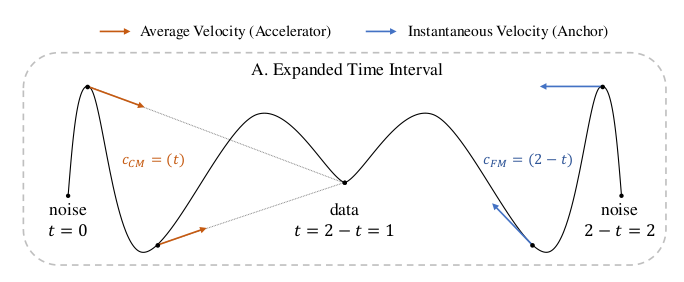
\includegraphics[width=0.6\textwidth]{figures/anchor_flows.png}
  \caption{Time representation for anchor and accelerator flows.}
  \label{fig:times}
\end{figure}

\noindent This work is comparable to the TrigFlow paper : it's a set of improvements to cosistency models, drawing inspiration from the Flow Matching paradigm. Authors even mention that TrigFlow eventually converges towards the same solution, but slower, and by chance. 

\subsection{Large Scale Diffusion Distillation via Score-Regularized Continuous-Time Consistency}
Authors of \cite{zheng2025largescalediffusiondistillation} propose a parallelized implementation of the Flash-Attention layer using JVP. This enables training of models with more than 10B parameters for large-scale video generation. Notably, they can parallelize training for batches of data $[B, H, L, C]$ (batch size, number of heads, sequence length and number of channels) when $L$ is large, such as in video generation.

Then, they introduce score-based regularization to mitigate the pitfalls of sCM. This regularization introduces a new loss:
\begin{align*}
    \mathcal{L}_{DMD}(\theta)  = \mathbb{E}\left[ \lVert \mathbf{x}_0 -sg\left(\mathbf{x}_0 - \frac{\mathbf{f}_{fake}(\mathbf{x}_t, t) - \mathbf{f}_{teacher}(\mathbf{x}_t, t)}{\frac{1}{N} \sum|\mathbf{x}_0 - \mathbf{f}_{teacher}(\mathbf{x}_t, t)|}\right)\rVert^2_2\right]
\end{align*}
\noindent where $\mathbf{f}_{fake}$ serves as a proxy student score by minimizing:
\begin{align*}
    \mathbb{E}\left[ \omega(t) \lVert \mathbf{f}_{fake}(\mathbf{x}_t, t) - \mathbf{x}_0 \rVert^2_2 \right]
\end{align*}

This is another paper that builds upon sCM. It is reserved for long-sequence output (with large $L$), typically video sampling. We will also have a large $L$ since we forecast the entire sampling trajectory. Probably, we could re-use the parallel JVP layer.